% !TEX root = main.tex

In the previous chapters, we discussed the requirements and support of
data- and compute-intensive workflows on high performance computing (HPC)
resources. When considering actual research, scientific projects require to
execute multiple workflows at scale and potentially for long period of time.
Usually, workflows are first developed, tested and executed for small scale
problems which can be verified theoretically. When ready, multiple workflows
are executed, potentially concurrently, at production scale for long periods
of time on the target HPC machine(s) while trying to achieve an objective.
This poses unprecedented computing challenges, shifting the problem from
enabling the effective and efficient execution of a single workflow at scale,
to managing the execution of a computational campaign.

The challenges users face when executing a computational campaign include, but
are not limited to, deciding an execution plan, submitting, executing and
monitoring workflows, and transferring data among resources. Workflow submission
requires users to have knowledge of submission systems, which generally differ
among HPC resources. Furthermore, users have to connect to those resources to
get information about the execution of workflows. Lastly, users have to
establish an execution plan which defines when each workflow will be executed
and on which HPC resource, with workflows potentially executing concurrently. A
campaign manager which, given a computational campaign and a set of resources,
creates an execution plan, submits, executes and monitors workflows on HPC
resources can address those challenges.

Existing campaign managers make assumptions about the resources and middleware
they are utilizing. In addition, they are monolithic software systems, despite
their modular design, and tend to be domain specific. For example,
PanDA~\cite{maeno2008panda}, Pegasus~\cite{deelman2015pegasus}, and
glideinWMS~\cite{sfiligoi2008glidein} are not easily extensible to use other
capabilities or runtime systems. QCFractal~\cite{qcfractal} is built to be
extensible and be able to interface with different workflow and workload
management systems, but remains domain specific.

In response to the limitations of existing campaign managers---monolithic
design, domain specific support, and dependence on specific resource and
middleware---we design and prototype a new campaign manager (CM). As our
CM has to support use cases from different scientific domains,
such as molecular dynamics, earth sciences and high energy physics on
potentially heterogeneous and diverse resources, the design and functionality
space grow exponentially. A prototype allows us to identify the most important
components and functionalities to support our use cases. Further, we can quickly
implement and test the CM without necessarily considering any
performance and data management requirements that may arise when executing an
actual campaign on actual production infrastructures. Finally, a prototype
allows us to tune parts of the CM with minimal engineering cost.

The CM prototype is domain agnostic as its design does not depend
on requirements from any specific scientific domain. In addition, our prototype
is designed by following the building blocks
approach~\cite{turilli2019middleware}. In this way, the prototype is agnostic
and makes no assumptions about the workflow management framework used to manage
the execution of individual workflows, as well as the type of resources used.

The chapter is organized as follows: \S~\ref{sec:cm_rw} discusses the current
solutions in executing computational campaigns. In \S~\ref{sec:cm_req}, we discuss the
supported use cases and the CM requirements.
\S~\ref{sec:cm_des} describes the building blocks approach and the design
of the CM. In \S~\ref{sec:cm_impl} we describe the
implementation of the CM prototype and we characterize its
baseline performance. We close the chapter with our conclusions in
Section~\ref{sec:cm_concl}.

\section{Related Work}

Currently, many software systems support computational campaigns. Among those,
PanDA~\cite{maeno2008panda}, DIRAC~\cite{casajus2010dirac},
QCFractal~\cite{qcfractal}, and glideinWMS~\cite{sfiligoi2008glidein} are the
ones with the widest adoption. These campaign managers, apart from
GlideInWMS~\cite{sfiligoi2008glidein}, are domain specific and make assumptions
about the underlying software stack and type of workflows to be executed. PanDA
WMS~\cite{maeno2008panda} mainly supports the distributed data analysis of data
produced by the ATLAS experiment~\cite{atlas} at the large hadron collider
(LHC). PanDA has been adapted to other use cases and projects, but it requires
major tailoring and dedicated support. This is also true for
DIRAC~\cite{tsaregorodtsev2003dirac}, which mainly supports the LHCb Monte Carlo
simulation production system at CERN. QCFractal~\cite{qcfractal} is a campaign
manager developed to execute large-scale quantum chemistry campaigns. It allows
users to define workflows based on the geometry of physical systems and execute
calculations, hiding the specifics of the software used.
GlideInWMS~\cite{sfiligoi2008glidein} is a more general purpose campaign manager
as it was specifically designed to support different use cases.

Existing campaign managers also support a plethora of computing resources,
including Grid resources, HPCs and Cloud. PanDA~\cite{maeno2008panda},
glideinWMS~\cite{sfiligoi2008glidein} and DIRAC~\cite{casajus2010dirac} mainly
support grid resources. PanDA has been extended to support
HPC~\cite{de2015future, de2016accelerating} and cloud
resources~\cite{de2016accelerating}, while glideinWMS~\cite{sfiligoi2008glidein}
supports only cloud resources. QCFractal~\cite{qcfractal} supports a set of
heterogeneous resources, including local campus clusters, and HPC and
cloud resources.

Workflow management frameworks such as Pegasus~\cite{deelman2015pegasus} and
Balsam~\cite{salim2019balsam} support the concurrent execution of multiple
workflows on HPC resources. Both frameworks allow users to submit multiple
workflows concurrently for execution but Balsam also provide multitenancy
capabilities, where multiple users can submit jobs for execution under the same
workflow. Despite this capabilities, both frameworks execute workflows as
independent entities but not as part of a computational campaign with a well
defined objective.

\section{Campaign Manager Requirements}
\label{sec:cm_req}

The space of data analysis of computational campaigns can be vast with different
scientific objectives, types and number of workflows and resources. We use three
real use cases with data analysis workflows to derive the requirements of the
CM prototype. The first use case supports quantum chemistry
campaigns (UC1), the second earth science (UC2) and the third data analysis
campaigns which analyze the data produced for the ATLAS experiment (UC3).

Quantum chemistry defines campaigns which execute workflows that perform
chemical computations on molecules to calculate their properties, e.g., energy.
These campaigns execute thousands of workflows, with up to 1000 executing at any
given point in time, on a number of resources~\cite{smith2020molssi}. Workflows
execution time varies between half-core hours up to 100-core hours, with
different levels of concurrency. In addition, users have access to resources
with several capabilities and not every workflow can be executed on every
resource. During the campaign definition, users may provide an initial workflow
priority and have to be sure that the campaign will finish within the given
resource allocation.

Earth science campaigns analyze imagery acquired via sensors from different
calendar years~\cite{paraskevakos2019workflow} to create time series of
ecological events, executing one workflow per imagery from a calendar year.
Their execution time varies from hours to a couple of days. Due to the volume of
the data, users have access to a small number of resources where imagery is
stored. While workflows analyze datasets based on the year they represent, a
specific execution order is not necessary as long as all datasets are analyzed.
The objective of this campaign is to analyze as many years of imagery as
possible, thus they target high throughput imagery per unit of time.

The third use case supports the execution of data analysis workflows from the
ATLAS experiment~\cite{atlas}. LHC produces data as particles collide inside its
detectors. These data are then analyzed by executing hundreds to thousands
workflows with different timescales and frequencies~\cite{borodin2015big}. In
addition, the analysis needs to happen within specific time boundaries, while
the detector is not operational. For example, one of the use cases described in
Ref.~\cite{borodin2015big} analyzes thousands of different datasets with
workflows running for months every yearly quarter. As a result, the objective of
this use case campaign is to finish all of its workflows within a specific
amount of time.

Based on these use cases, we derive a set of functional requirements for the
CM prototype. Table~\ref{tab:fun_reqs} shows a summary of the
functional requirements. The table defines a requirement identification number,
states the requirement and provides a description of each requirement. In
addition to this information, the table shows from which use case the
requirement is derived with ``G'' being a requirement that supports all three
use cases.

\begin{table}[t]
    \centering
    \scriptsize
    \begin{tabular}{@{}p{1.5cm}|p{2.8cm}p{1.5cm}p{6cm}@{}}
        \toprule
        \textbf{REQ ID} &\textbf{Requirement Algorithm} &\textbf{Use Case} & \textbf{Description} \\
        \midrule
         1 &
         Support campaign with O(1k) workflows &
         UC1 &
         The CM should be able to support campaigns with order of thousand workflows.
         Planning, execution and adaptation should be able to execute with such a campaign.\\
         2 &
         The CM should support at least two different planning algorithms. &
         G &
         Users/developers should be able to easily extend the planning capabilities with algorithms.\\
         3 &
         Support from 1 up to 100 resources &
         UC1-UC2 &
         The CM should be able to execute workflows on multiple resources concurrently.
         These resources can either be actual or emulated resources.\\
         4 &
         Plan should be derived for heterogeneous and homogeneous static resources in 5 minutes &
         G &
         The plan should be derived as soon as the user provides a campaign description.
         Plan should be derived in less than 5 minutes.\\
         5 &
         Plan should be derived and adapted for heterogeneous/homogeneous dynamic resources in 5 minutes &
         UC1 &
         The plan should be derived as soon as the user provides a campaign description.
         Plan should be derived in less than 5 minutes.
         In case the plan needs to be adapted, it should be adapted in less than 5 minutes.\\
         6 &
         Interface with different WMFs &
         G &
         The CM should be able to interface with different WMFs based on the specifics of the campaign. \\
         7 &
         Early bind workflows to resources &
         UC1 &
         The user may need to bind workflows to specific resources before executing the campaign.\\
         8 &
         Campaign objective is configurable &
         UC1 &
         While the campaign is executing, the objective may be adjusted based on user preferences.\\
         9 &
         Update the campaign during runtime &
         UC1-UC2 &
         The user may want to update the campaign while it is executing to add/remove workflows.\\
         10 &
         Resources may be added or removed during runtime &
         UC1 &
         The user may want to add/remove resources, she has gained/lost access to.\\
        \bottomrule
    \end{tabular}
    \caption{Campaign manager functional requirements.\label{tab:fun_reqs}}
\end{table}

\section{Campaign Manager Design}
\label{sec:cm_des}

This section discusses the design principles (\S\ref{ssec:building_blocks}) and
the architecture (\S\ref{ssec:cm_arch}) of the campaign manager prototype.

\subsection{Building Blocks Design Approach}
\label{ssec:building_blocks}

The building blocks approach, as described in Ref.~\cite{turilli2019middleware},
defines four design principles for software systems. Those are self-sufficiency,
interoperability, composability, and extensibility. Adhering to those principles
during the design and implementation phase of a software system allows for
greater software sustainability. In addition, it allows users not to tailor
their solutions to a specific software ecosystem and take full advantage of the
plethora of software that supports scientific computing.

Self-sufficiency and interoperability describe the characteristics of software
entities and functionalities. The entities are enough to stand alone and can
be reduced to a specific abstraction. The functionalities of each building
block are specific to the block and do not overlap with other blocks. As a
result, the CM design defines a set of components and that allow
it to execute a campaign to HPC resources without providing capabilities to
execute the individual workflows of the campaign or acquire the necessary
resources.

Composability and extensibility describe the communication and coordination
between building blocks and the generality of the generality of the blocks
components respectively. Blocks communicate information about their state,
events and errors. Based on this information alone building blocks are
coordinating with each other. As a result, the CM uses only the
state of the workflow execution to create the campaign state. Furthermore, its
components are designed to be general enough so that they can extended and
interface with different workflow execution engines as well as software
systems that execute computational campaigns.

\subsection{Campaign Manager Components}
\label{ssec:cm_arch}

We define three components as part of the CM prototype (see
Figure~\ref{fig:refarch}):
\begin{inparaenum}[(1)]
    \item a Planner;
    \item an Enactor; and
    \item a Bookkeeper.
\end{inparaenum}
Workflow execution will be managed by an existing workflow management framework
(WMF) on HPC resources. Each of these components supports a basic functionality
of the CM, such as executing individual workflows and monitoring
the campaign.

\begin{figure*}[t]
    \centering
    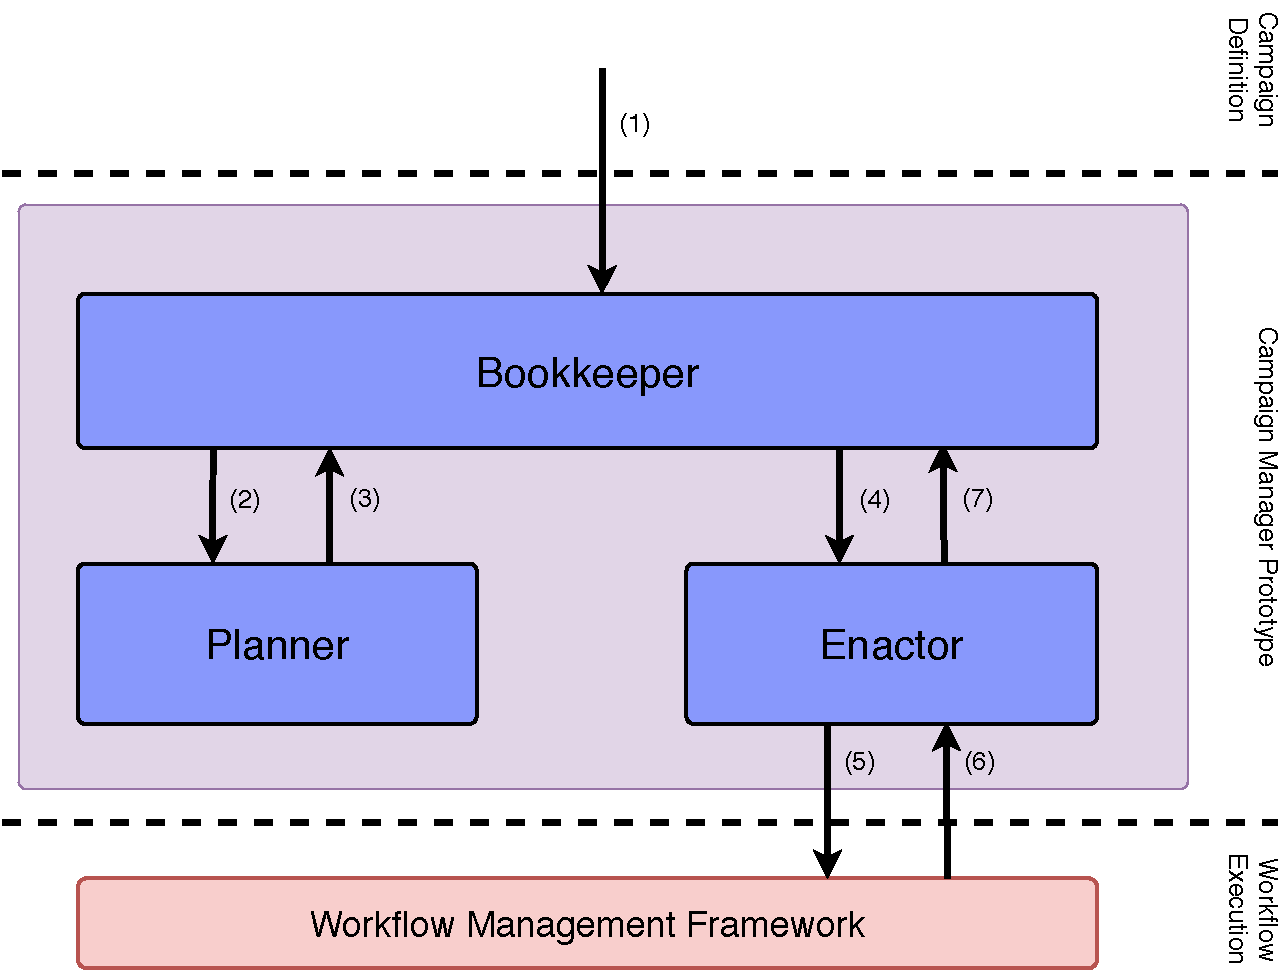
\includegraphics[width=.75\textwidth]{figures/manager/CEM_design.pdf}
    \caption{Reference Architecture of a Campaign Manager. Basic components of
        Campaign Manager (CM): (a) Planner, (b) Enactor and (c) Bookkeeper. CM
        communicates decisions to Workflows Management Framework. CM
        communicates with HPCs to execute parts of the
        campaign.}\label{fig:refarch}
\end{figure*}

The Planner component derives an execution plan based on a planning algorithm
and calculates the makespan for a campaign on a specific set of resources. The
Planner receives information about available resources and the workflows of the
campaign from the Bookkeeper component. The Planner does not adhere to a
specific planning algorithm, allowing different algorithms to be used, based on
the campaign's requirements and objective.

The Bookkeeper component is responsible for monitoring the execution of the
campaign. This component holds information about the state of the campaign, the
execution plan, the availability of resources, and the campaign's objective. The
state of the campaign is based on information about workflow execution provided
by the Enactor component. In addition, the Bookkeeper knows the state of the
resources utilized by the campaign at runtime and the state of the resources
that are planned to be used. Based on this information, the Bookkeeper checks
whether the campaign's objective can be achieved. Bookkeeper requests the
Planner to update the plan when changes in the campaign happen that
affect the effectiveness of a current plan or make the objective not achievable.
For example, the availability of one or more resources can change during
runtime, requiring a revision of the execution plan.

The Enactor component executes the campaign's workflows by interfacing with a
workflow management system (WMF). The Enactor receives a set of workflows from
the Bookkeeper, along with the resources on which the workflows will execute at
a given point in time. Based on this information, the Enactor submits the
workflows to the WMF for execution.

Initially, the Bookkeeper receives the description of a campaign
(Figure~\ref{fig:refarch} step 1) and passes information about resources and
workflows to the Planner (Figure~\ref{fig:refarch} step 2). As soon as a plan is
calculated, it is passed to the Bookkeeper (Figure~\ref{fig:refarch} step 3).
Then, the Bookkeeper passes the workflows and resources descriptions to the
Enactor (Figure~\ref{fig:refarch} step 4) and the Enactor passes that
information to the selected WMF for execution (Figure~\ref{fig:refarch} step 5).
When a workflow finishes to execute, the Enactor gets notified
(Figure~\ref{fig:refarch} step 6) and informs the Bookkeeper
(Figure~\ref{fig:refarch} step 7). Steps 4, 5, 6 and 7 repeat until all the
workflows have finished executing.

\section{Prototype Implementation and Performance Evaluation}
\label{sec:cm_impl}

Consistent with the design presented in~\S\ref{sec:cm_des}, we define three main
classes to implement the CM prototype. The Bookkeeper class
implements the capabilities of the Bookkeeper component, the Enactor class
interacts with a selected workflow engine to execute workflows on resources, and
the Planner class implements planning algorithms. In addition, the prototype
defines a state model for the campaign and the workflows.
Figure~\ref{fig:rcm_class_diagram} shows the class diagram of the prototype.
Each class also defines a set of data structures to support the execution of campaigns.

\begin{figure*}[t]
    \centering
    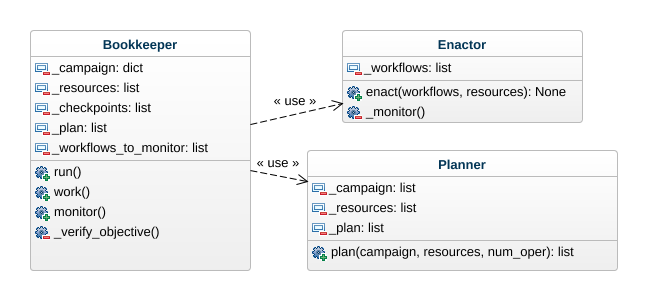
\includegraphics[width=.95\textwidth]{figures/manager/class_diagram.png}
    \caption{Class diagram of campaign manager prototype}\label{fig:rcm_class_diagram}
\end{figure*}

The states models provide information about the state of the execution. The
campaign state model (Figure~\ref{fig:CampaignStates}) has six states: (1)
\textit{new}, (2) \textit{planning}, (3) \textit{executing}, and (4)
\textit{done} or (5) \textit{canceled} or (6) \textit{failed}. A campaign is
considered \textit{new} when it is defined and no further action is taken. The
campaign transitions to the \textit{planning} state when a plan for its
execution is derived. As soon as the execution of the campaign starts, the state
of the campaign transitions to \textit{executing}. The final states are possible
termination states. When the campaign execution ends and the campaign objective
is achieved, the campaign transitions to the \textit{done} state. If the
objective cannot be achieved or there is a failure during the execution, the
state of the campaign changes to \textit{failed}. Lastly, the campaign state
goes to \textit{canceled} when the user cancels the execution of the campaign.
The code of the prototype is publicly available on Github~\cite{cm_git}.

\begin{figure*}[t]
    \centering
    \begin{subfigure}[b]{0.45\textwidth}
        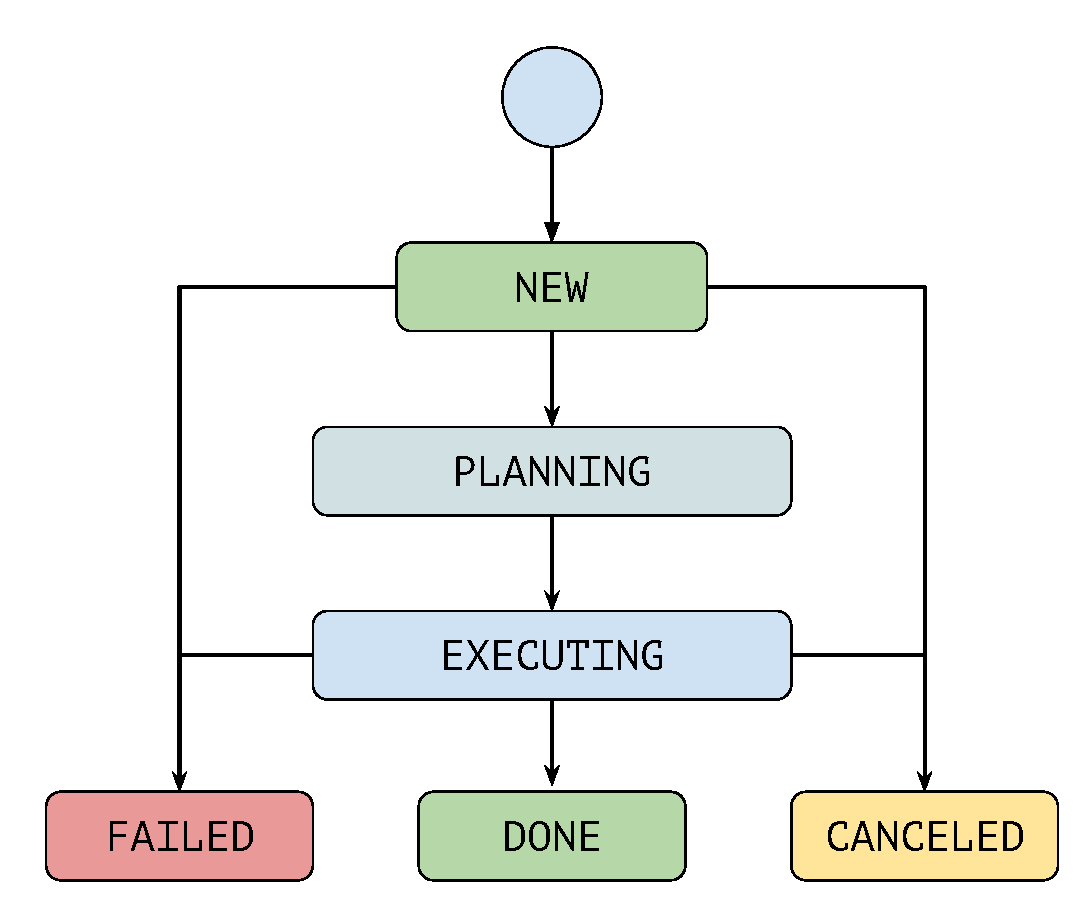
\includegraphics[width=.95\textwidth]{figures/manager/campaign-state-model.pdf}
        \caption{}
        \label{fig:CampaignStates}
    \end{subfigure}
    ~
    \begin{subfigure}[b]{0.45\textwidth}
        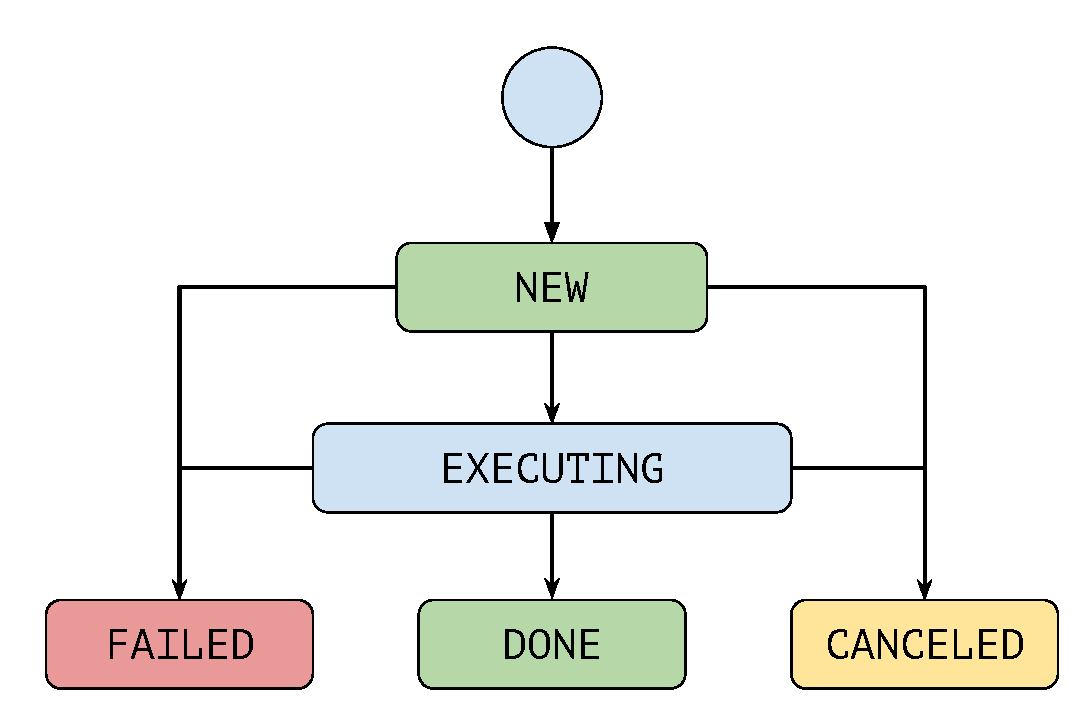
\includegraphics[width=.95\textwidth]{figures/manager/workflow-state-model.pdf}
        \caption{}
        \label{fig:WorkflowStates}
    \end{subfigure}
    \caption{State diagrams for : ~\ref{fig:CampaignStates}) a campaign;~\ref{fig:WorkflowStates}) each workflow of a campaign.}
    \label{fig:StateDiagrams}
\end{figure*}

Similar to the campaign state model, the workflows state model
(Figure~\ref{fig:WorkflowStates}) defines five states: (1) \textit{new}, (2)
\textit{executing}, and (3) \textit{done} or (4) \textit{canceled} or (5)
\textit{failed}. A workflow is in the \textit{new} state when it is received by
the Bookkeeper and transitions to the \textit{executing} state when the Enactor
submits the workflow for execution to the selected WMF. The workflow transitions
to one of the final states---\textit{done}, \textit{canceled} or
\textit{failed}---based on the final state the workflow management system
reports.

The Bookkeeper class defines several methods to execute a campaign. The most
important ones are: \textit{run}, \textit{work} and \textit{monitor}. The
\textit{run} method initializes the campaign state to \textit{new} and sets up
the environment for executing the campaign. \textit{Work} calls the Planner to
produce a plan transitioning the state of the campaign to \textit{planning}.
After a plan is produced, \textit{work} calls \textit{\_verify\_objective} to
verify if the objective of the campaign can be achieved, and either starts
submitting workflows to the Enactor or transitions the campaign to the
\textit{failed} state. In addition, \textit{work} pushes the submitted workflows
to a data structure that the \textit{monitor} method reads. The \textit{monitor}
method checks the state of the workflow which are executing and receives
information from the Enactor via callbacks.

The Planner and Enactor classes define the methods for planning the execution
of a campaign, executing workflows on resource and monitoring their execution.
The Planner defines a \textit{plan} method which implements a planning
algorithm and returns a plan. The Enactor's \textit{enact} method submits a
workflow to the selected WMF. The \textit{monitor} method of the Enactor
checks periodically the state of the workflows that are executing and pushes
state updates to the Bookkeeper via a callback.

\begin{figure*}[t]
    \centering
    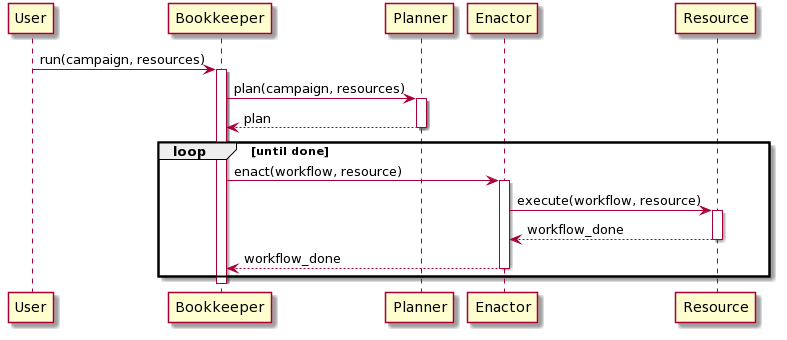
\includegraphics[width=.85\textwidth]{figures/manager/rcm_seq.png}
    \caption{Sequence diagram for executing a computational campaign through the campaign manager prototype}
    \label{fig:seq_diag}
\end{figure*}

Figure~\ref{fig:seq_diag} shows the sequence diagram of the execution. Before
the execution of a campaign, the Bookkeeper gets as input a campaign (a set of
workflows) and a set of resources. As the user requests to execute the campaign,
the Bookkeeper passes to the Planner the information it needs. When the plan is
ready, the execution of the campaign begins with the Bookkeeper passing a
workflow to the Enactor, along with a list of resources to use for the
execution. As the Enactor executes the workflow, it pushes state updates to the
Bookkeeper via callbacks. The Bookkeeper continues to pass workflows to the
Enactor as resources become available, until there are no more workflows to execute.

Instead of an actual workflow management framework (WMF), the Enactor utilizes a
modified version of the workload emulator proposed in
Ref.~\cite{balasubramanian2019programming}. The emulator allows us to define
heterogeneous resources and emulate the execution of workloads on those
resources. A workload is a set of independent tasks that can be executed 
concurrently. We modified the emulator to emulate the execution of a campaign 
which is a set of independent workflows.  In addition, we extended the emulator 
execution capabilities with SimPy~\cite{simpy}, a discrete time simulator. 
SimPy executes discrete simulations by producing events as time progresses. 
These events provide information about which workflows are executing or have 
finished to execute. The Enactor polls these events and pushes to the 
Bookkeeper the state of each workflow. As a result, we are able to simulate the 
execution of a campaign and validate the correctness of our design and its 
implementation.

\begin{figure*}[t]
    \centering
    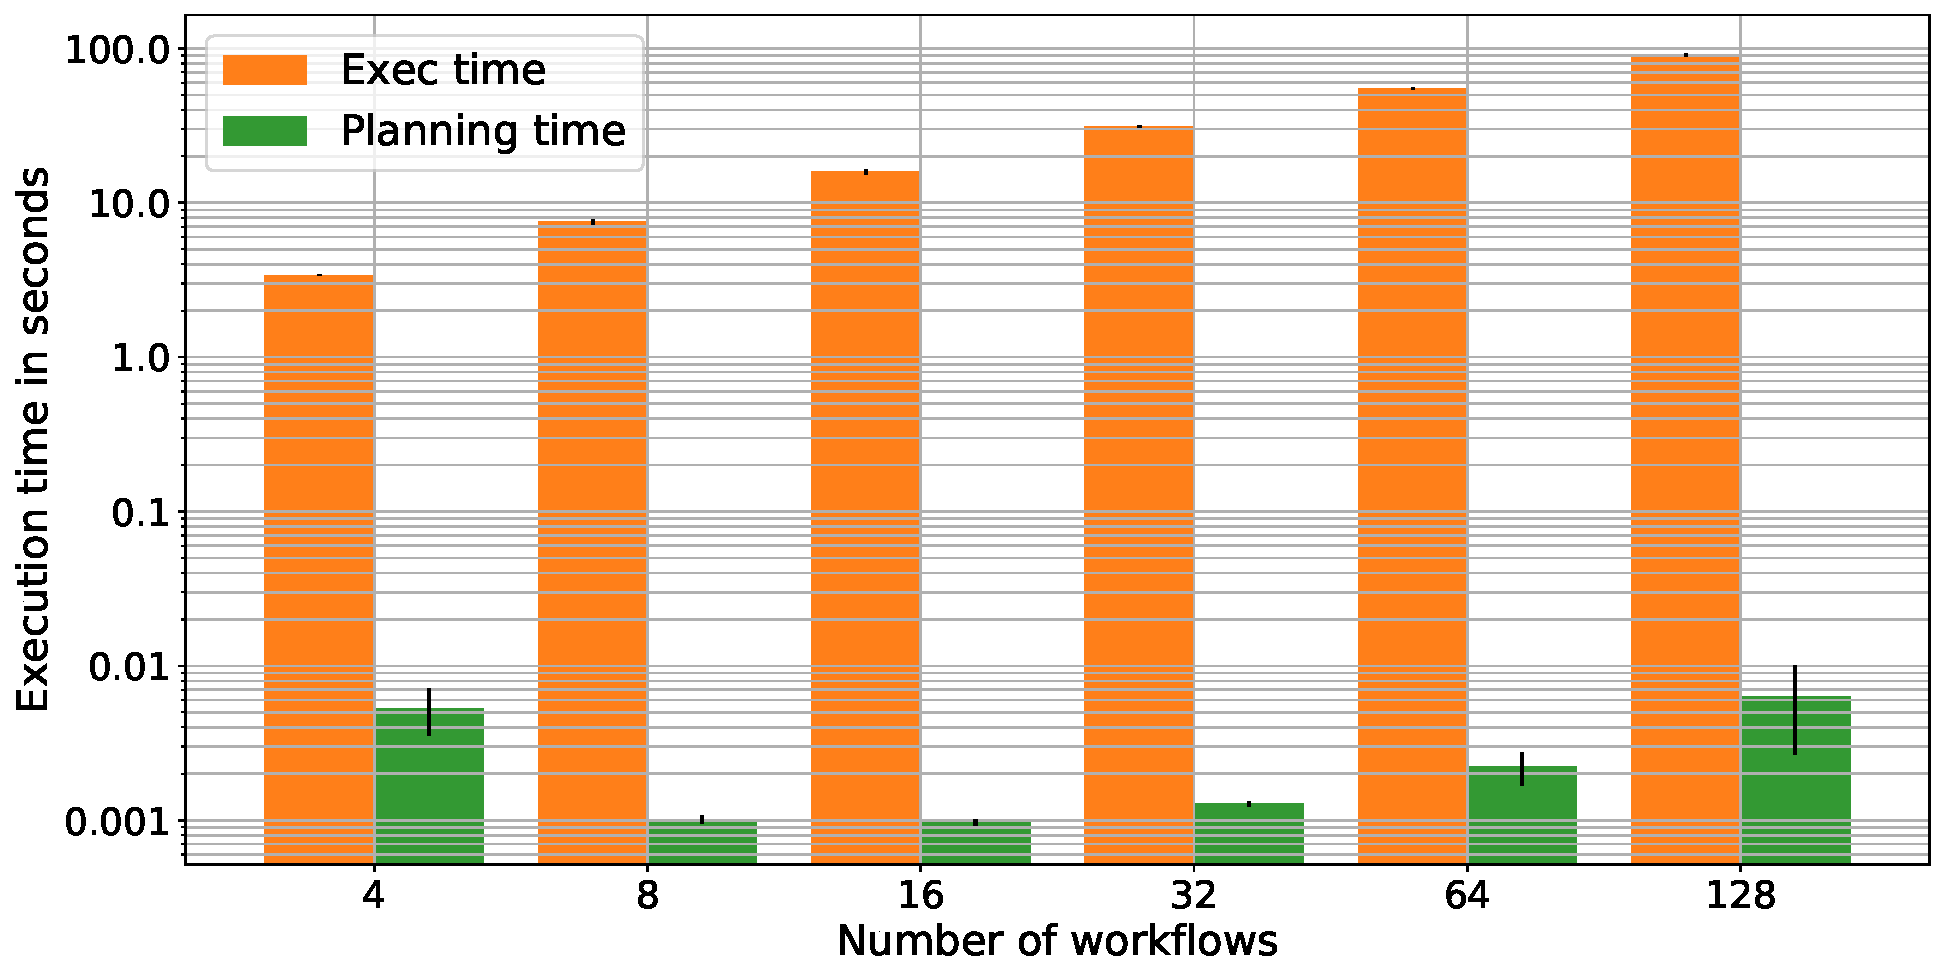
\includegraphics[width=.95\textwidth]{figures/manager/SimTimeWork.pdf}
    \caption{Execution time of simulating the execution of computational campaign with different number of workflows on different number of resources, $N_R$.}
    \label{fig:cm_char}
\end{figure*}

We validated the correctness of our design by executing campaigns of different
sizes on different number of resources. We provided the prototype with a
campaign, a set of resources and an execution plan. We then check that the
workflows of the campaign were executed as expected and in a viable amount of
time, as shown in Figure~\ref{fig:cm_char}. We observed that the execution time
of the simulation increases when more than 64
resources are utilized concurrently. Both the Enactor and the Bookkeeper have
monitoring methods that traverse the list of executing workflows. In
addition, the Enactor uses callbacks to inform the Bookkeeper about the state of
the workflows. Above 64 resources, these operations start to dominate the
execution time of the simulation. The prototype executed 128
workflows on 128 resources in $\approx$15 minutes, an amount of time we considered acceptable for experimental purposes.
% and thus we conclude that this increase will not affect the execution of an
% actual campaign. As a result, we conclude that the design and functionalities
% of the prototype satisfy the requirements and correctly execute a
% computational campaign.


\mtnote{Validation: do the prototype+emulator do what they are supposed to do?
    E.g., given a campaign and an unfeasable amount of resources, do they deem
    the campaign unplannable? Are workflows marked as failed/cancelled as per
    the given specification? Given a feasable amount of resources, do they deem
    the campaign plannable? If you have time/data/tests I would write a
    paragraph along these lines.}

\section{Conclusions}
\label{sec:cm_concl}
In this chapter, we motivated, discussed and validated a prototype for a
software system that supports the execution of computational campaigns on HPC
resources based on a set of use cases. We described the design and the basic
components of the CM, a Bookkeeper, a Planner and an Enactor.
Based on the selected design, we implemented a software prototype that simulates
the execution of a campaign on resources. The prototype allows us to understand
and correctly implement the necessary functionality of the CM.

The CM produces an execution plan for a computational via the Planner class. The
Planner is able to support several planning algorithms. Although using any
planning algorithm would satisfy the requirement of creating an execution plan, 
it is necessary to utilize an algorithm that is able to achieve the campaigns 
objective. In the next chapter, we investigate planning algorithms and evaluate 
the plans they produce for executing computational campaigns.
